\clearpage
\textbf{ГЛАВА 1. Теоретические основы генерации случайных чисел}

\begin{enumerate}
\def\labelenumi{\arabic{enumi}.}
\item
  \textbf{Основные понятия и определения.}
\end{enumerate}

\textbf{Случайная последовательность} -- последовательность данных, в
которой отсутствуют статистические закономерности, а каждый следующий
элемент невозможно предсказать, зная предыдущие. С точки зрения
достоверности случайности последовательности разделяются на истинно
случайные и псевдослучайные.

\textbf{Истинно случайные последовательности (ИСП)} -- это
представленные в виде последовательности случайные числа. Случайные
числа являются реализацией некоторой случайной величины. Случайная
величина -- это функция над пространством элементарных событий,
принимающая вещественные значения с некоторыми вероятностями. Таким
образом, истинно случайные последовательности -- это последовательности
статистически независимых друг от друга величин, принимающих в
результате опыта одно из множества заранее непредсказуемых значений.
Связь между значениями случайной величины и соответствующими
вероятностями описывается законом распределения, который задается с
помощью функции распределения или связанной с ней функцией плотности
вероятности. Истинно случайные последовательности должны обладать
равномерным распределением.

Однако на практике далеко не всегда возможно непосредственно
использовать выходные данные источников истинно случайных чисел. Поэтому
обычно приходится использовать так называемые псевдослучайные
последовательности. \textbf{Псевдослучайная последовательность (ПСП)} --
это последовательность, состоящая из псевдослучайных двоичных чисел,
получаемых с помощью заданного детерминированного алгоритма, но
применяемых в качестве случайных. При этом обычно алгоритмы получения
ПСП используют специальное случайное начальное значение, или «зерно»
(seed). Для того чтобы ПСП могли использоваться в качестве случайных
последовательностей, они должны по статистическим свойствам быть близки
к ИСП.

\textbf{Энтропия} -- это мера хаотичности информации, неопределённости
или непредсказуемости. В контексте данной темы будет чаще встречаться
понятие источника энтропии, то есть источника, используемого для
получения случайной величины, которая необходима генераторам истинно
случайных последовательностей для формирования случайных чисел.

\textbf{Корреляция} -- это наличие связи между значениями выходной
последовательности, особенно показательна корелляция между соседними или
близкими по времени значениями. Другими словами, если два бита (или
числа), которые идут друг за другом, не полностью независимы друг от
друга, говорят, что между ними есть корреляция. Это плохо для ГСЧ,
поскольку идеальная случайная последовательность должна быть независимой
и равномерно распределённой -- т.е. каждый бит должен быть
непредсказуемым, независимо от предыдущих.

Коэффициент корреляции для удобства исследования случайных
последовтельностей может быть представлен в следующем виде{[}2{]}:

\[Corr(X_{t},X_{t + \tau}) = \frac{E\left\lbrack (X_{t} - \mu)(X_{t + \tau} - \mu) \right\rbrack}{\sigma^{2}}\]

где:

\begin{quote}
\(X_{t}\) --- значение на момент времени t,

τ --- сдвиг (лаг) по времени,

\emph{μ} --- математическое ожидание,

\(\sigma^{2}\) -- дисперсия.
\end{quote}

Если корреляция больше нуля при малых τ, это значит, что соседние
значения похожи --- и сигнал не полностью случаен.

\textbf{Спектральная плотность} (спектральная плотность мощности шума
или просто плотность шума) --- это количественная характеристика,
описывающая, как энергия случайного сигнала (в виде шума) распределена
по частотам. В контексте генераторов истинно случайных чисел,
спектральная плотность показывает, на каких частотах сосредоточена
энтропия, и является важным инструментом анализа качества и природы
случайности сигнала.

Спектральная плотность мощности случайного сигнала x(t) определяется
как{[}2{]}:

\[S_{x}(f) = {\lim_{T \rightarrow \infty}{\frac{1}{T}\left| \int_{\frac{- T}{2}}^{\frac{T}{2}}{x(t)e^{2\pi ift}}dt \right|}}^{2}\]

В контексте источников энтропии, плоский (частотно-независимый) спектр
\emph{S(f) = const} соответствует белому шуму --- идеальному случаю,
когда энтропия равномерно распределена по частотам.

\begin{enumerate}
\def\labelenumi{\arabic{enumi}.}
\setcounter{enumi}{1}
\item
  \textbf{Классификация генераторов случайных чисел.}
\end{enumerate}

Генераторы случайных чисел разделяются на две основные категории:
истинные генераторы случайных чисел (ГИСП) и псевдослучайные генераторы
чисел (ГПСП). ГИСП создают случайные числа, опираясь на физические
источники, к примеру, шум от тепловых, атмосферных или радиоактивных
явлений. С другой стороны, ГПСП генерируют числа детерминированно на
основе начального значения, которое должно быть трудно предсказуемым и
безопасным. Если кто-либо извне получает доступ к нему или может влиять
на его генерацию, то он может предсказать вывод ГПСП, что будет являться
нарушением безопасности. Схема общей структуры модуля ГИСП представлена
на рисунке 1{[}9{]}{[}12{]}.

\noindent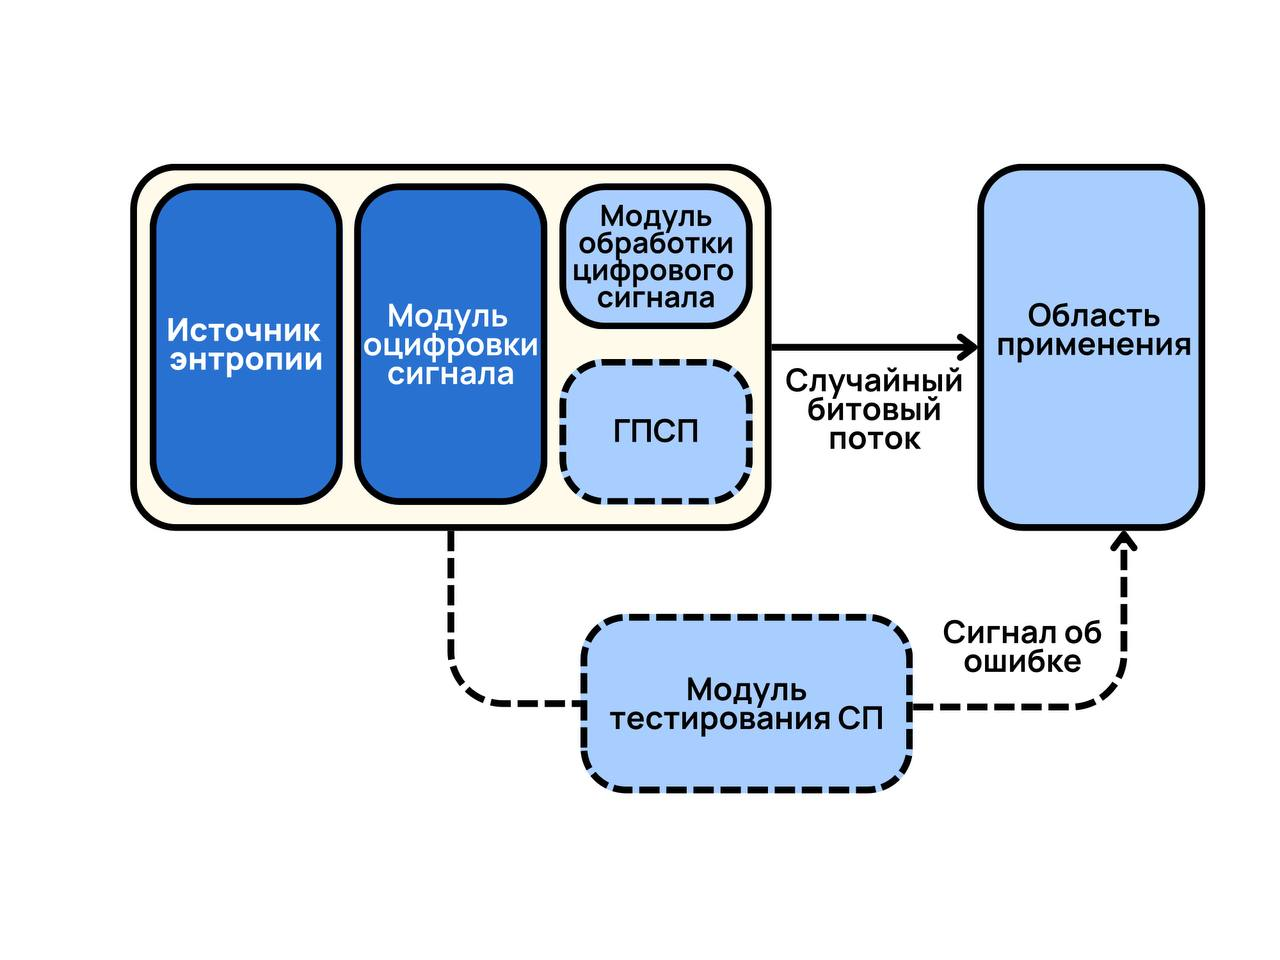
\includegraphics[width=\linewidth,keepaspectratio]{pandoc_media/media/image1.png}

Рисунок 1

Генератор псевдослучайных последовательностей (ГПСП) -- это функция,
которая принимает короткое случайное начальное значение и выдает более
длинную последовательность бит, которая кажется случайной.
Криптографически стойкий генератор псевдослучайных чисел (КСГПСП)
обладает свойствами стойкости к криптоанализу и является важным
средством в обеспечении безопасности криптографических систем, таких как
шифрование данных, создание ключей и другие приложения, где требуется
случайность с высоким уровнем безопасности. Для обеспечения
криптографической безопасности вывод ГПСП должен быть вычислительно
неотличим от случайной строки. Это означает, что при наличии короткого
префикса последовательности должно быть вычислительно невозможно
предсказать оставшуюся часть последовательности без знания начального
значения.

Кроме этого, возможно выделить гибридный тип генератора случайных чисел,
который совмещает в себе ГИСП, для формирования начального значения
(seed), и ГПСП, который использует полученное начальное значение для
дальнейших генераций, что позволяет такому классу ГСП поддерживать
достаточно высокий уровень криптографической безопасности и скорости
генерации.

Также ГСП можно классифицировать по методам генерации случайных
последовательностей{[}4{]}:

Табличные генераторы. Используют уже готовые таблицы, из которых
получают случайные последовательности. Их главное преимущество
заключается в высокой скорости работы, а недостаток в большом объёме
хранимых данных для достаточной безопасности сформированной
последовательности.

Алгоритмические генераторы. Подобные генераторы используют определенные
математические формулы для создания последовательностей случайных чисел.
Конечно, они могут генерировать исключительно псевдослучайные
последовательности. Их реализация при приближении к истинно случайным
величинам требует значительных вычислительных ресурсов компьютера.

Физические генераторы. ГСП данного типа используют внешние явления и
воздействия в качестве источника случайных величин, опираясь на
показания датчиков или индикаторов, фиксирующих какой-либо случайный
физический процесс, либо получая информацию о естественно происходящем
или искусственно вызванном хаотическом явлении иными способами.
Простейшими примерами физического генератора случайных
последовательностей могут служить монета (игра в «орла» и «решку») либо
игральные кости. О других наиболее практико-применимых источниках
энтропии для физических ГСП будет сказано позже.

\begin{enumerate}
\def\labelenumi{\arabic{enumi}.}
\setcounter{enumi}{2}
\item
  \textbf{Методы оценки случайности последовательностей}
\end{enumerate}

Случайные последовательности, созданные как физическими, так и
алгоритмическими генераторами в особенности требуют оценки качества их
действительной случайности. Существует несколько способов тестирования
случайных последовательностей:

Графические тесты. Свойства последовательностей отображаются в виде
графических зависимостей, по виду которых делают выводы о свойствах
исследуемой последовательности. К данной категории можно отнести
следующие тесты: гистограмма распределения элементов последовательности,
распределение на плоскости, проверка на монотонность и т.д. На рисунке 2
представлен пример графического теста «распределение на плоскости».
Слева результат тестирования отрицательный, справа --
положительный{[}10{]}.

\noindent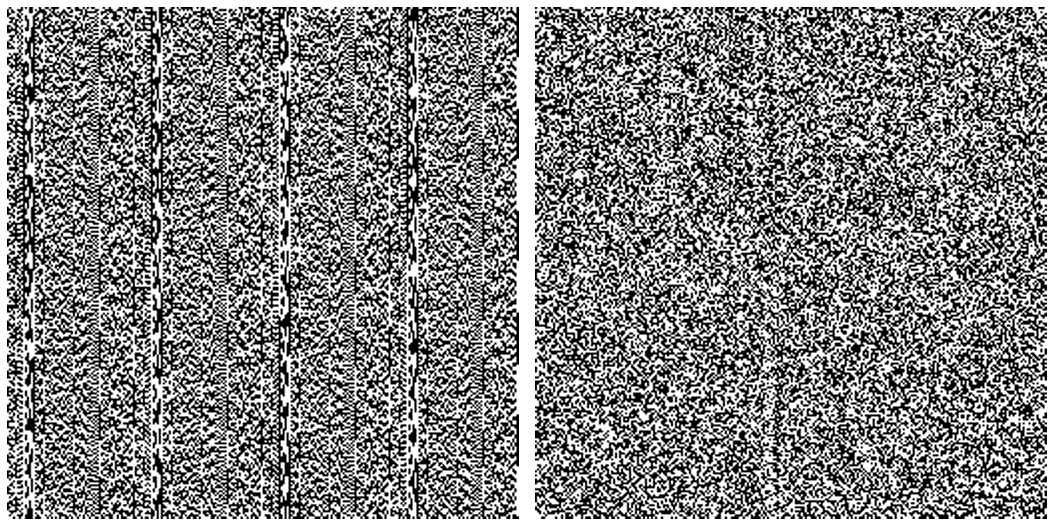
\includegraphics[width=\linewidth,keepaspectratio]{pandoc_media/media/image2.png}

Рисунок 2.

Статистические тесты. Основным критерием, применяемым для анализа
качества генераторов случайных чисел, являются статистические тесты. Они
проверяют соответствие последовательностей математическим свойствам
случайных данных. В основе тестов лежит понятие нулевой гипотезы. За
нулевую гипотезу принимается предположение, что последовательность
является истинно случайной. Следовательно, если нулевая гипотеза верна,
то наш генератор производит достаточно хорошие случайные числа.
Существует 4 варианта возможных выводов по результатам тестов{[}3{]}:

\begin{enumerate}
\def\labelenumi{\arabic{enumi}.}
\item
  Сделан вывод о том, что последовательность случайна, и это верный
  вывод
\item
  Сделан вывод о том, что последовательность не случайна, хотя она была
  на самом деле случайна. Такие ошибки называют ошибками первого рода
\item
  Последовательность признана случайной, хотя на самом деле таковой не
  является. Такие ошибки называют ошибками второго рода
\item
  Последовательность справедливо отбракована
\end{enumerate}

Наиболее популярные пакеты статистических тестов случайных и
псевдослучайных последовательностей {[}6{]} представлены в таблице 1.

Таблица 1.

{\def\LTcaptype{none} % do not increment counter
\begin{longtable}[]{@{}|%
  >{\raggedright\arraybackslash}p{(\linewidth - 8\tabcolsep - 5\arrayrulewidth) * \real{0.0520}}|%
  >{\raggedright\arraybackslash}p{(\linewidth - 8\tabcolsep - 5\arrayrulewidth) * \real{0.1909}}|%
  >{\raggedright\arraybackslash}p{(\linewidth - 8\tabcolsep - 5\arrayrulewidth) * \real{0.3721}}|%
  >{\raggedright\arraybackslash}p{(\linewidth - 8\tabcolsep - 5\arrayrulewidth) * \real{0.3757}}|@{}}
\hline
\begin{minipage}[b]{\hsize}\raggedright
№
\end{minipage} & \begin{minipage}[b]{\hsize}\raggedright
Пакеты статистических тестов
\end{minipage} & \begin{minipage}[b]{\hsize}\raggedright
Тестирование СП длины до 300 бит
\end{minipage} & \begin{minipage}[b]{\hsize}\raggedright
Тестирование СП длины порядка 10⁶ бит
\end{minipage} \\ \hline
\endhead
\endlastfoot
1 & Тесты Д. Кнута & -- & \begin{minipage}[t]{\hsize}\raggedright• критерий частот\\
• критерий серий\\
• критерий «максимум-t»\\
• критерий монотонности\strut
\end{minipage} \\ \hline
2 & NIST STS & \begin{minipage}[t]{\hsize}\raggedright
• частотный побитовый тест (Frequency Test)\\
• частотный блочный тест (Frequency Test within a Block)\\
• тест на последовательность одинаковых бит (Runs Test)\\
• тест на совпадение неперекрывающихся шаблонов (Non-overlapping
Template Matching Test)\\
• тест на периодичность (Serial Test)\\
• тест рангов бинарных матриц (Binary Matrix Rank Test)\\
• тест приблизительной энтропии (Approximate Entropy Test)\\
• тест кумулятивных сумм (Cumulative Sums (Cusum) Test)\\
• тест на самую длинную последовательность «1» в блоке (Test for the
Longest Run of Ones in a Block)\strut
\end{minipage} & \begin{minipage}[t]{\hsize}\raggedright
• частотный блочный тест (Frequency Test within a Block)\\
• тест на последовательность одинаковых бит (Runs Test)\\
• тест на совпадение перекрывающихся шаблонов (Overlapping Template
Matching Test)\\
• тест на периодичность (Serial Test)\\
• тест на линейную сложность (Linear Complexity Test)\\
• спектральный тест (Discrete Fourier Transform Test)\\
• универсальный статистический тест Маурера (Maurer Universal Test)\\
• тест рангов бинарных матриц (Binary Matrix Rank Test)\\
• тест приблизительной энтропии (Approximate Entropy Test)\\
• тест на произвольные проходы (Random Excursions Test)\\
• другой тест произвольные проходы (Random Excursions Variant Test)\\
• тест на самую длинную последовательность «1» в блоке (Test for the
Longest Run of Ones in a Block)\strut
\end{minipage} \\ \hline
3 & DIEHARD & -- & • проверка промежутков между днями рождений (The
Birthday Spacing Test) \\ \hline
4 & TestU01 & \begin{minipage}[t]{\hsize}\raggedright
• тест веса Хэмминга (Hamming Weight Test)\\
• тест автокорреляции (Autocorrelation)\\
• тест случайных проходов (Random Walk Test)\\
• тест на самую длинную последовательность «1» в блоке (Longest Run of
1\textquotesingle s Test)\strut
\end{minipage} & \begin{minipage}[t]{\hsize}\raggedright
• тест веса Хэмминга (Hamming Weight Test)\\
• тест серий и разрывов (Run and Gap Test)\\
• тест сложности последовательности на основе алгоритма Лемпела-Зива
(Lempel-Ziv Complexity Test)\\
• тест автокорреляции (Autocorrelations Test)\\
• тест на самую длинную последовательность «1» в блоке (Longest Run of
1\textquotesingle s Test)\\
• CAT тест (CAT Test)\strut
\end{minipage} \\ \hline
5 & Crypt-XS & \begin{minipage}[t]{\hsize}\raggedright
• тест частот (Frequency Test)\\
• тест бинарной производной (Binary Derivative Test)\strut
\end{minipage} & • тест сложности последовательности (Complexity
Test) \\ \hline
\end{longtable}
}

Наиболее подходящими тестами для оценки СП в выбранной теме будут NIST
STS (Statistical Test Suite), так как они в совокупности обладают
достаточной строгостью и полнотой оценки, имеют свой стандарт NIST SP
(Special Publication) 800-22, который является достаточно известным в
сфере криптографии и наиболее часто применяются для оценки именно
физических ГСП{[}8{]}. Для общего ознакомления каждый из статистических
тестов пакета NIST STS с кратким описанием приведены в виде таблицы в
приложении 1.

Для физических ГСП особенно важны спектральный тест (№12) и тест Маурера
(№13){[}5{]}. Спектральный тест анализирует последовательность в
частотной области с помощью преобразования Фурье, чтобы обнаружить
скрытые периодичности или аномальные пики. Подобный тест способен
выявить периодические паттерны, которые могут появляться в физическом
ГСП по нескольким причинам, таким как колебания напряжения в схеме,
влияние внешних электромагнитных помех и дефекты датчиков (например,
шумового диода). Спектральный тест обнаруживает такие скрытые частотные
компоненты, которые не видны в статистических тестах на битовом уровне.

Тест Маурера оценивает алгоритмическую сложность последовательности,
проверяя, насколько она «несжимаема». Случайные данные не должны
допускать оптимизации при сжатии. Он особенно важен для проверки
физических генераторов потому, что физические процессы (например, шум в
транзисторах) иногда порождают статистически случайные, но
алгоритмически простые последовательности. Тест Маурера способен выявить
такие случаи. Кроме этого, генераторы с низкой энтропией (например,
из-за «залипания» датчика в определённых состояниях) проваливают этот
тест.

Дополнительное подтверждение необходимости тестирования физических
генераторов тестами 12 и 13 вытекает из того, что стандарт NIST SP
800-22 рекомендует эти тесты для аппаратных генераторов, используемых в
криптографии. Практический пример: квантовые ГСП обязательно проверяют
спектральным тестом на предмет квантовых корреляций.

